\documentclass[conference,letterpaper]{IEEEtran}

\usepackage{amsmath}
\usepackage{graphics}
\usepackage{graphicx}
\usepackage[english]{babel}

\bibliographystyle{/home/rsheissa/papers/midwest_2006/IEEEtran}

\begin{document}

% paper title
\title{A Synthesis Tool for Low-noise Nullor-based Amplifiers}

% author names and affiliations
\author{Roberto Casta\~neda-Sheissa, Arturo Sarmiento-Reyes, Luis Hern\'andez-Mart\'inez\\ National Institute for Astrophysics, Optics and Electronics\\
Electronics Department, CAD Group\\ P.O. Box 51, 72000, Puebla, Pue., Mexico}

% make the title area
\maketitle

\begin{abstract}
The applications for low noise amplifers (LNA's) ranges from wideband-ultrawideband radio, microwave signals to cell-phone designs. In the structured design, the process to create an amplifier starts by establishing an ideal solution provided by an ideal element, named nullor, which fulfils a set of specifications.\\
A LNA can be designed, in first instance, employing a nullor representing an ideal active gain, i.e. the plant to be controlled by the feedback network which is usually constituted by passive components. This work shows the automation of the nullor synthesis for a low-noise amplifier based on the structured design guidelines producing, as a result, an optimised bias value.
\end{abstract}

\section{Introduction}
Low noise amplifiers can be seen as systems where noise and gain are taken in equal concern. The noise contribution by this kind of amplifier is carefully handled. In radio receivers the low-noise amplifier is usually placed at the first block. It can be seen as a stage that takes a signal and condition it to be further processed.

Besides the traditional design that resorts to the knowledge previously acquired by the designer, there is an alternative to perform analog design. Structured design \cite{verhoeven} is a methodology that resorts to the idea of first define an ideal solution. Once this ideal solution is established it is transformed by means of assumptions and rules provided by the electronics theory. Its aim is to optimise aspects like noise, distortion and bandwidth by applying the concept of orthogonality \cite{nordholt}. Orthogonality lets the designer to focus on only one design aspect (noise, distortion or bandwidth) at a time \cite{stoffels}.

This paper is organised as follows:

\begin{itemize}
\item Nullor-based amplifiers. Here the basics about nullor and its applications is outlined.
\item Noise synthesis equations. The equations which the synthesis tool are based.
\item Tool structure. How the tool works.
\item Example. An example is provided to verify the tool.
\end{itemize}

\section{Nullor-based amplifiers}
As previously stated the nullor is the key piece for the structure design methodology. This ideal device represents the active part of the amplifier. It can be seen as a two port device composed by two elements: {\bf the nullator} which is placed at the input port and {\bf the norator} located at the output port. The transmission matrix (also known as chain-matrix) is given as \cite{carlin,moschytz}:

\begin{equation}\label{eq:abcd}
{K}
=
\left [ \begin{array}{cc}
\frac{1}{\mu}& \frac{1}{\gamma} \\\\
\frac{1}{\zeta}& \frac{1}{\beta}
\end{array}
\right ]
=
\left [ \begin{array}{cc}
0 & 0 \\ 0 & 0
\end{array}
\right ]
\end{equation}

From the transmission matrix it can be seen that the nullor is a device that possesses infinite gains for the transfer relationships, voltage ($\mu$), current ($\alpha$), transconductance ($\gamma$) and transimpedance ($\zeta$). Therefore the ideality of nullor is demonstrated.

\begin{figure}[b]
	\centering
	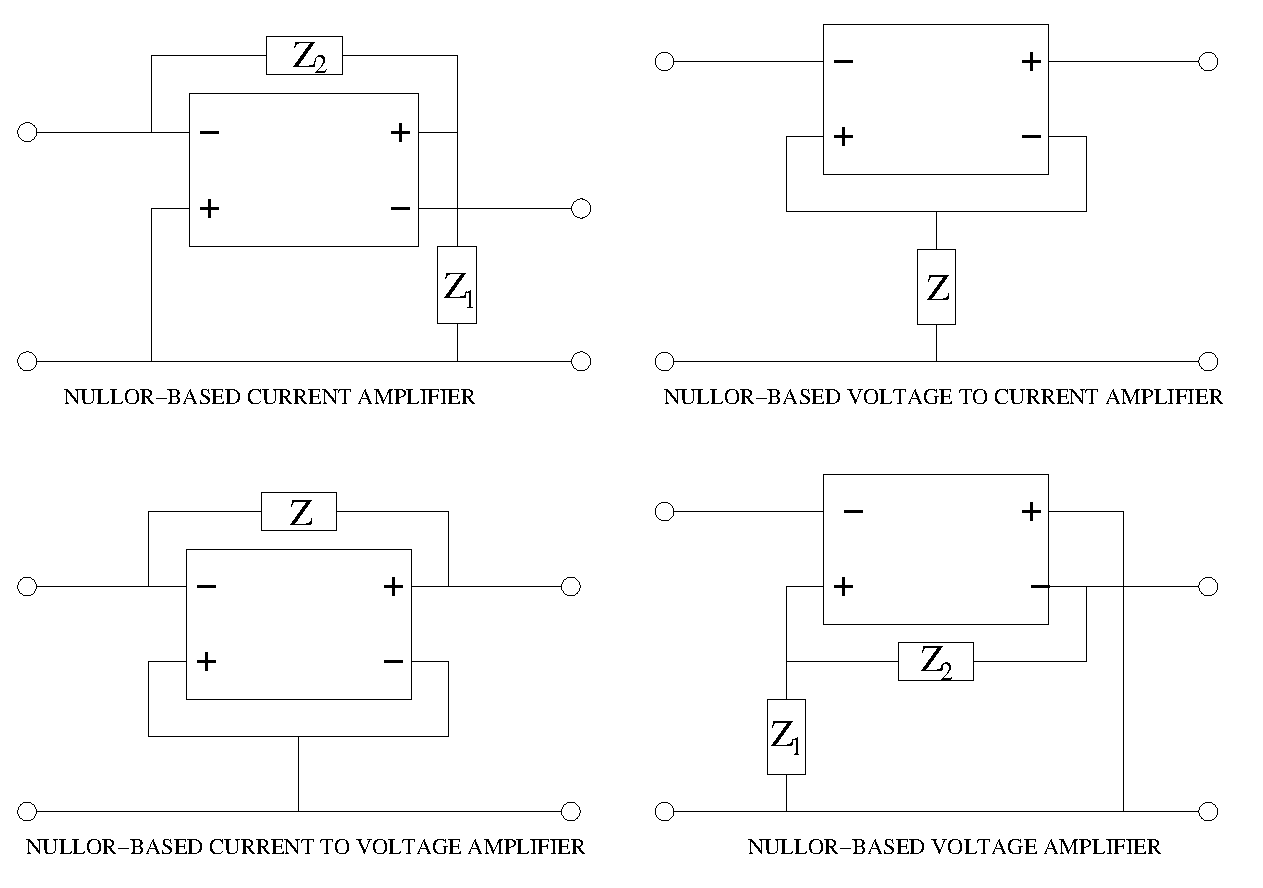
\includegraphics[scale=.4]{figures/nullor_based.eps}
	\caption{Single-loop Amplifiers.}
	\label{figure2}
\end{figure} 

\begin{figure}
	\centering
	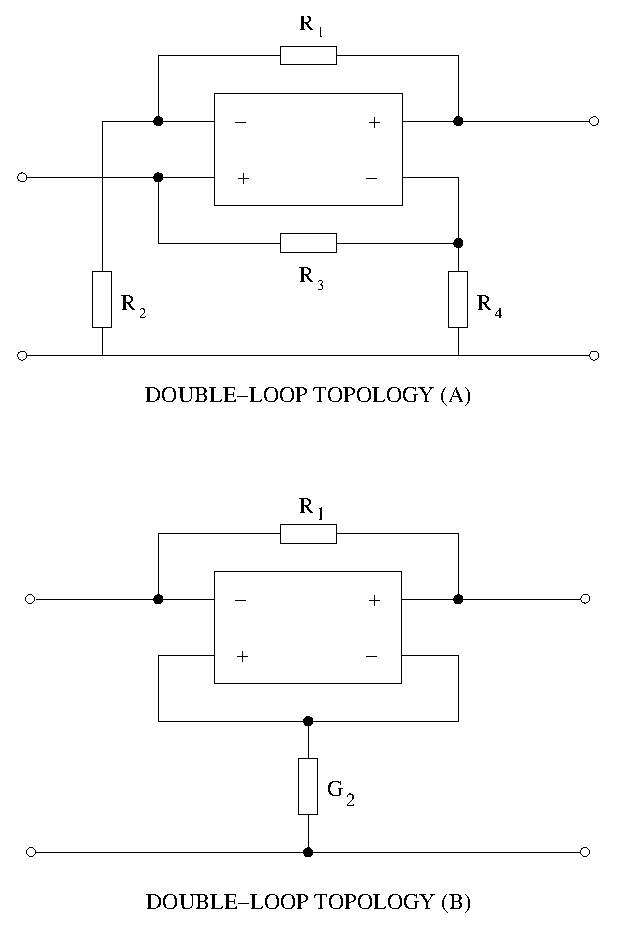
\includegraphics[scale=.55]{figures/basic_two_loops.eps}
	\caption{Double-loop Amplifiers.}
	\label{figure3}
\end{figure}

If a feedback network is attached to the nullor then an ideal amplifier is created. The basic configurations are named {\it single-loop amplifiers}. This feedback network is a passive network since the nullor is the active part. The Figure \ref{figure2} shows these configurations. It is possible to combine the single-loop configurations and the {\it double-loop configurations} are created. When the voltage amplifier is combined with the current amplifier a {\it double-loop topology (A)} amplifier is created. Combining the transconductance and transimpedance amplifiers create the {\it double-loop topology (B)} \cite{nordholt,stoffels}.

Topology (B) can achieve all four kinds of transfers (voltage, current, transconductance and transimpedance), while Topology (A) can achieve all but the transconductance.

\section{Noise Synthesis Equations}
Noise can be regarded in terms of power spectral densities originated from the passive network and the synthesised nullor. Because structured design uses power spectral densities for noise calculations it is necessary to convert the noise figure term for the active devices into a noise voltage and current model, this method is explained in \cite{ott}.

The method to obtain the equivalent input noise sources for the single-loop topologies is detailed in \cite{sarmiento}, for the two-loop topologies a similar approach is used although it results rather cumbersome. The overall noise of the amplifier consists of two contributions. The first contribution comes from the feedback network, while the second contribution comes from the active devices.

\subsection{Equations at Nullor Level}
Noise equations for the single-loop topologies (Figure \ref{figure2}) are:

\begin{itemize}
\item Voltage Amplifier.
\begin{equation}
\begin{split}
u_{n,v_{total}}=u_{ns}+u_{nn}+\biggl(R_s+\frac{R_1R_2}{R_1+R_2}\biggr)i_{nn}+\\
+\biggl(\frac{R_2}{R_1+R_2}\biggr)u_{nR_1}+\biggl(\frac{R_1}{R_1+R_2}\biggr)u_{nR_2}
\label{eq:noise_volt}
\end{split}
\end{equation}
\item Transadmittance Amplifier.
\begin{equation}
u_{n,v_{total}}=u_{ns}+u_{nn}+\Bigl(R_s+R\Bigr)i_{nn}+\Bigl(R\Bigr)i_{nR}
\label{eq:noise_transadm}
\end{equation}
\item Transimpedance Amplifier.
\begin{equation}
i_{n,i_{total}}={i_{ns}}+{i_{nn}}+{\biggl(\frac{1}{R_s}+\frac{1}{R}\biggr)u_{nn}}+{\biggl(\frac{1}{R}\biggr)u_{nR}}
\end{equation}
\item Current Amplifier.
\begin{equation}
\begin{split}
i_{n,i_{total}}=i_{ns}+i_{nn}+\biggl(\frac{1}{R_s}+\frac{1}{R_1+R_2}\biggr)u_{nn}+\\
\biggl(\frac{R_2}{R_1+R_2}\biggr)i_{nR_2}+\biggl(\frac{R_1}{R_1+R_2}\biggr)i_{nR_1}
\end{split}
\end{equation}
\end{itemize}

Equations for the double-loop topologies (Figure \ref{figure3}) are:
\begin{itemize}
\item Voltage-driven Double-loop Amplifier (A).
\begin{equation}
\begin{split}
u_{n,v_{total}(A)}=u_{ns}+u_{nn}+{\qquad}{\qquad}{\qquad}{\qquad}{\quad}\\
+\biggl(R_s+R_2+\frac{R_SR_2}{R_3+R_4}\biggr)i_{nn}+{\qquad}\\
+\biggl(\frac{R_2}{R_1+R_2}+\frac{R_S(R_3+R_4)}{(R_1+R_2)(R_3+R_4)}\biggr)u_{nR_1}+\\
+\biggl(1+\frac{R_s}{R_3+R_4}\biggr)u_{nR_2}+\biggl(\frac{R_S}{R_3+R_4}\biggr)u_{nR_3}+\\
+\biggl(\frac{R_S}{R_3+R_4}\biggr)u_{nR_4}{\qquad}{\qquad}{\qquad}{\qquad}{\qquad}{\quad}
\end{split}
\end{equation}

\item Current-driven Double-loop Amplifier (A).
\begin{equation}
\begin{split}
i_{n,i_{total}(A)}=i_{ns}+i_{nn}+\biggl(G_S+\frac{1}{R_3+R_4}\biggr)u_{nn}+\;\\
+\biggl(\frac{R_1R_2G_S}{R_1+R_2}+\frac{R_1R_2+R_1R_4}{(R_1+R_2)(R_3+R_4)}\biggr)i_{nR_1}+\;\;\;\;\\
+\biggl(R_2G_S+\frac{R_2}{R_3+R_4}\biggr)i_{nR_2}+{\qquad}{\qquad}{\qquad}{\quad}\;\\
+\biggl(\frac{R_3}{R_3+R_4}\biggr)i_{nR_3}+\biggl(\frac{R_4}{R_3+R_4}\biggr)i_{nR_4}{\qquad}{\qquad}\!
\end{split}
\end{equation}

\item Voltage-driven Double-loop Amplifier (B).
\begin{equation}
\begin{split}
u_{n,v_{total}(B)}=u_{ns}+u_{nn}++\biggl(R_S+\frac{R_S+R}{1-GR}\biggr)i_{nn}+\\
+\biggl(\frac{1+GR_S}{1-GR}\biggr)u_{nR}+\biggl(\frac{G(R+R_S)}{1-GR}\biggr)u_{nG}{\qquad}{\quad}
\end{split}
\end{equation}

\item Current-driven Double-loop Amplifier (B).
\begin{equation}
\begin{split}
i_{n,i_{total}(B)}=i_{ns}+i_{nn}+\biggl(G_S+\frac{G_S+G}{1-GR}\biggr)u_{nn}+\\
+\biggl(\frac{R(G_S+G)}{1-GR}\biggr)i_{nR}+\biggl(\frac{1+G_SR}{1-GR}\biggr)i_{nG}{\quad}{\quad}{\quad}\negthickspace
\end{split}
\end{equation}
\end{itemize}

\subsection{Equations for Single BJT Devices}
The nullor has to be synthesised by active devices, such as bipolar or MOS transistors. In similar way it is necessary to obtain the noise synthesis equations for these active devices. Spectral noise equations for BJT's depend on the way the transistor is connected as replacement of the nullor, i.e. the type of transistor configuration.

The spectral density noise equations for BJT devices employed to synthesise the nullor are:

\begin{itemize}
\item Common Emitter
\end{itemize}

\begin{equation}
\begin{split}
u_n=4kTr_b+\biggl(\frac{1}{gm}\biggr)2qIc\\
i_n=2qIb+\biggl(\frac{1}{\beta}\biggr)2qIc
\end{split}
\end{equation}

\begin{itemize}
\item Common Base
\end{itemize}

\begin{equation}
\begin{split}
u_n=\biggl(\frac{g_mr_o}{1+g_mr_o}\biggr)4kTr_b+\biggl(\frac{r_o}{1+g_mr_o}\biggr)2qIc\\
i_n=\biggl(\frac{1}{r_{\pi}+{\beta}r_0}\biggr)4kTrb+\biggl(\frac{r_o}{r_{\pi}+{\beta}r_o}\biggr)2qIc+2qIb
\end{split}
\end{equation}

\begin{itemize}
\item Common Collector
\end{itemize}

\begin{equation}
\begin{split}
u_n=4kTr_b+\biggl(\frac{r_{\pi}}{1+{\beta}}\biggr)2qIc+\biggl(\frac{r_{\pi}}{1+{\beta}}\biggr)2qIb\\
i_n=\biggl(\frac{1}{1+g_mr_{\pi}}\biggr)2qIc+\biggl(\frac{g_mr_{\pi}}{1+g_mr_{\pi}}\biggr)2qIb
\end{split}
\end{equation}

\section{Tool Structure}
Once defined the overall noise behaviour of an amplifier by its appropriate synthesis equation, it is now possible to define a general structure for a synthesis tool due to the modular structure provided by the structured design methodology, it is possible to translate this structure into an automated process \cite{stoffels} or by applying the object oriented concepts \cite{booch} to develop a computer program. Unlike some other efforts to automate the design process (\cite{stoffels}, \cite{nordholt}), the developed tool does not resort to a special description language. The basic structure is shown in Figure \ref{figure11}.

\begin{figure}
	\centering
	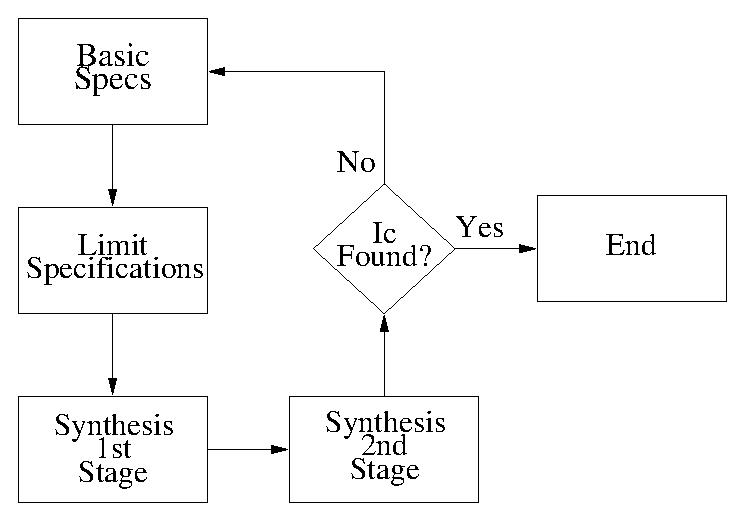
\includegraphics[scale=.5]{figures/tool_diagram.eps}
	\caption{Synthesis tool block diagram.}
	\label{figure11}
\end{figure}

The {\it basic spec} block is the stage to define basic specs like:

\begin{itemize}
\item Amplifier type (voltage, current, transadmittance, transimpedance).
\item Topology (single-loop, double-loop).
\item Gain.
\item Source impedance type and value.
\item Load impedance type and value.
\item Signal level.
\end{itemize}

{\it Limit specifications} is a stage where user specifies three values: distortion,  bandwidth, and noise constraints.

The {\it synthesis 1st stage} is the first step of the overall amplifier synthesis, that is, the feedback-network and source noise contributions are calculated. For the current and voltage amplifiers, based on gain value and configuration, optimal feedback resistors values are calculated. These values along with their related calculated noise are displayed. This provides the noise that the active device (or devices) that synthesises the nullor should accomplish.

Next is {\it synthesis 2nd stage} now that desired noise for the active device is known. At this stage user must select a model and configurations for the nullor to be synthesised. Once device model and configuration have been defined, the process of searching a valid range of Ic-bias is started. This range implies the value of collector current that fulfil the noise specification of the active part according to the synthesis equation for each transistor configuration.

Since this tool is aimed to have the minimum user intervention possible, the structure for the synthesis tool follows a wizard-oriented criterion. The wizard, NOMAD --Noise Optimisation in Modern Amplifier Design -- consists of a series of windows enabling each of the blocks described above. Figure \ref{figure4} shows the first window of the wizard used to enter the first group of specs. Figure \ref{figure5} shows the window for entering the specification for distortion, bandwidth and noise. Noise values can be given in two different units. Noise figure value is given in decibel units while spectral density is given by $\frac{V}{\sqrt{Hz}}$ or $\frac{A}{\sqrt{Hz}}$.

The tool has been developed in C++ for the backend, while the graphical user interface is programmed in Qt. The tool is aimed to run under Linux/Solaris without any constraints for special libraries. 

\begin{figure}
	\centering
	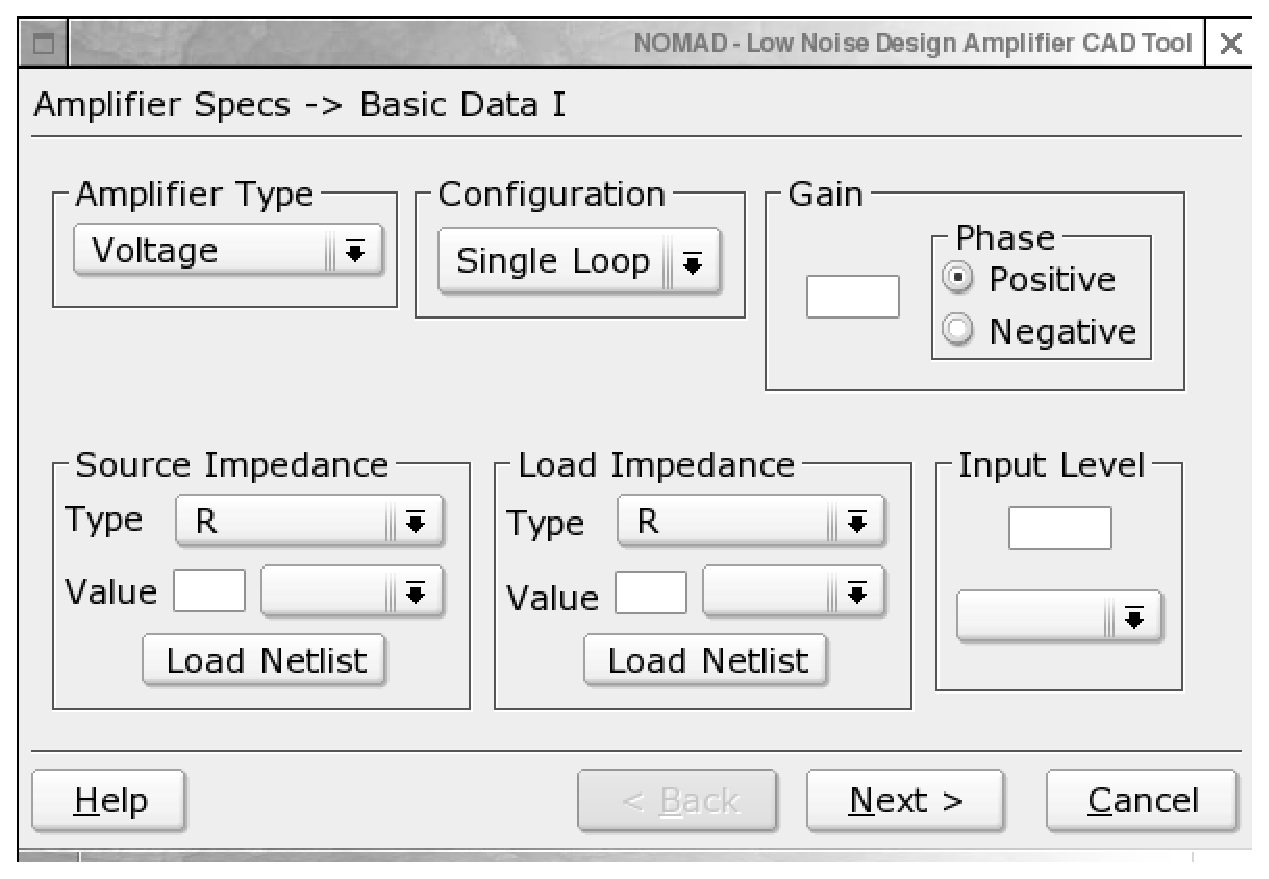
\includegraphics[scale=.3]{figures/descad_1.eps}
	\caption{First window for NOMAD wizard.}
	\label{figure4}
\end{figure}

\begin{figure}
	\centering
	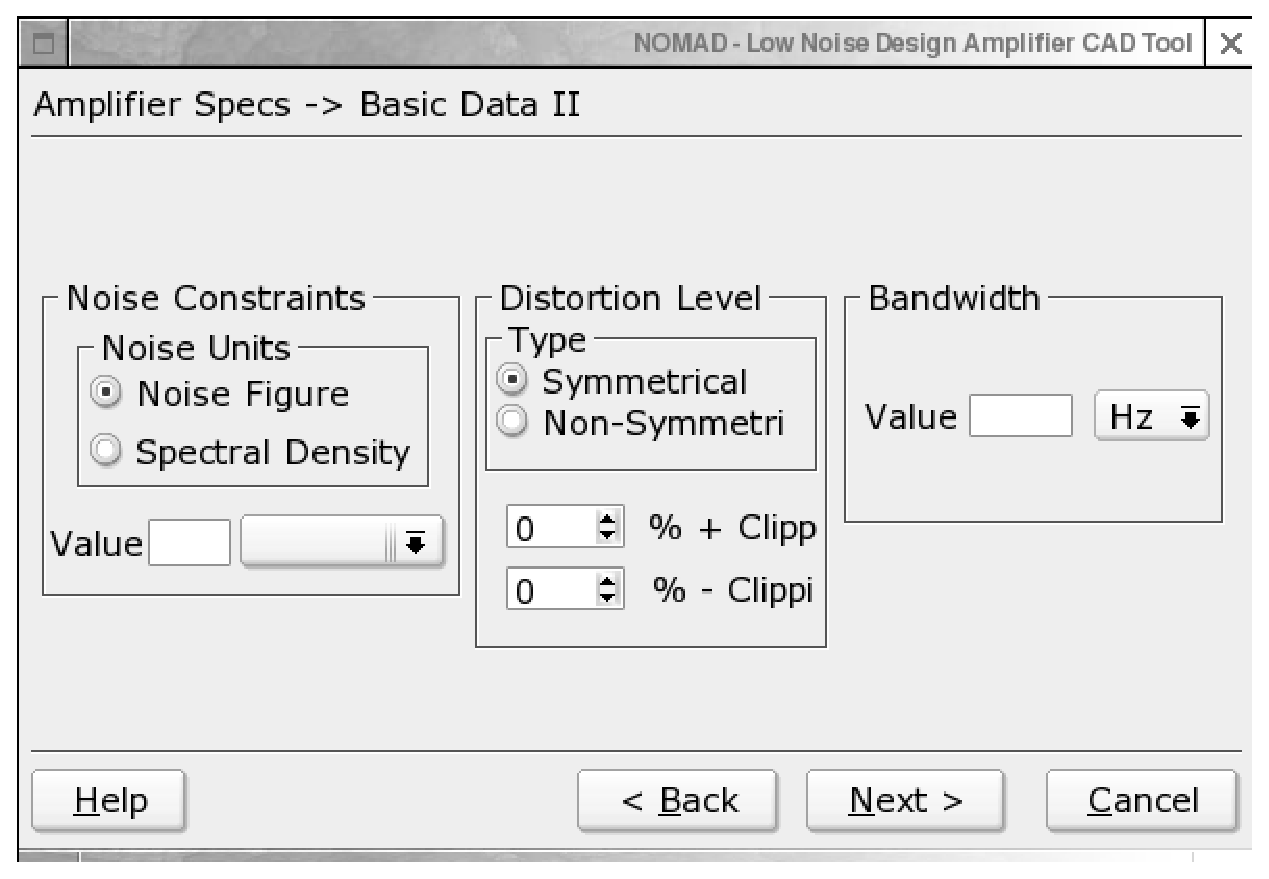
\includegraphics[scale=.3]{figures/descad_2.eps}
	\caption{Second window for NOMAD wizard.}
	\label{figure5}
\end{figure}

\section{Example}
A design example is provided in order to show the function of the tool. The amplifier to be designed must fulfil these specs:

\begin{itemize}
\item Type = Voltage Amplifier
\item Configuration = Single Loop
\item Source Impedance Type = Resistive
\item Source Impedance= 100 $\Omega$
\item Gain = 10 (20 dB)
\item Noise Figure = 2 dB
\item BW = 450 MHz
\end{itemize}

The calculated values for the feedback network are:
\begin{itemize}
\item R1 = 9 $\Omega$
\item R2 = 81 $\Omega$
\end{itemize}

Noise generated by feedback network and source are:
\begin{itemize}
\item Feedback Network Noise = 1.343E-19 $\frac{V^2}{Hz}$
\item Source Noise = 1.658E-18 $\frac{V^2}{Hz}$
\end{itemize}

For the active device these are the values:
\begin{itemize}
\item Model = BFR520
\item Configuration = Common Emitter
\item Bias Value = 340 ${\mu}A$
\item Noise Accomplished = 8.161E-19 $\frac{V^2}{Hz}$
\item Noise To Accomplish = 8.224E-19 $\frac{V^2}{Hz}$
\end{itemize}

In order to verify if the design has fulfilled the specs, the resulting amplifier is simulated in APLAC. The schema is shown in Figure \ref{figure8}. The nullor is replaced by an ideal op-amp, though this element is not a nullor, its behaviour is the closest to it. Figure \ref{figure9} shows that bias value for the BFR520 is the optimum to obtain the lowest noise figure. Figure \ref{figure10} shows the noise behaviour against frequency.

\begin{figure}
	\centering
	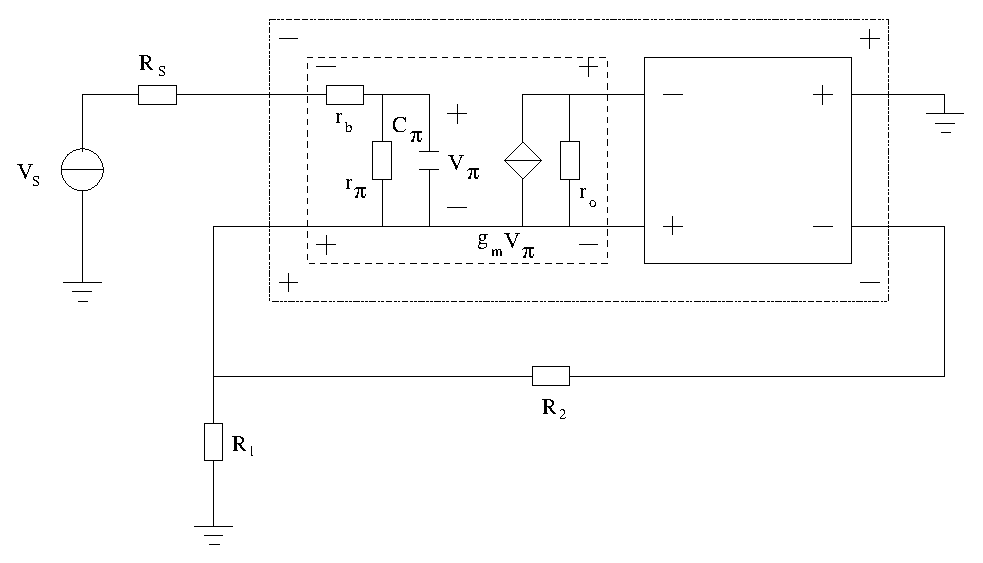
\includegraphics[scale=.4]{figures/amp_simulation.eps}
	\caption{Schema to simulate the nullor implementation.}
	\label{figure8}
\end{figure}

\begin{figure}
	\centering
	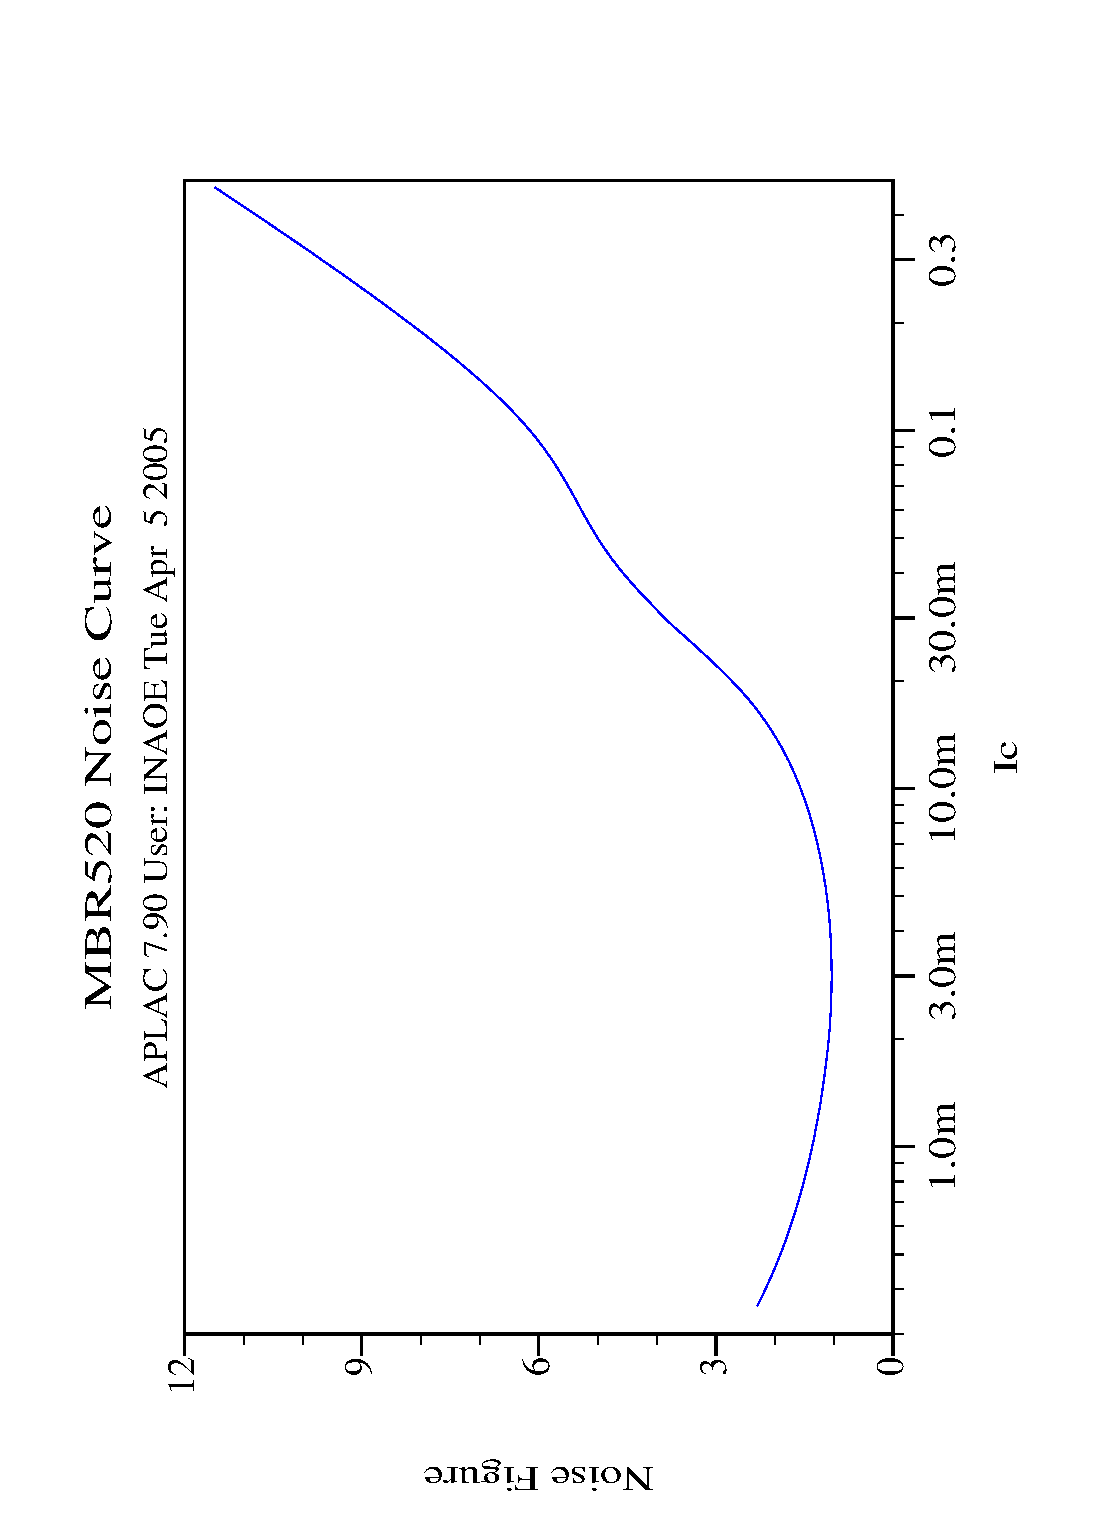
\includegraphics[scale=.3, angle=270]{figures/mbr520_noisecurves.eps}
	\caption{Noise figure versus collector current.}
	\label{figure9}
\end{figure}

\begin{figure}
	\centering
	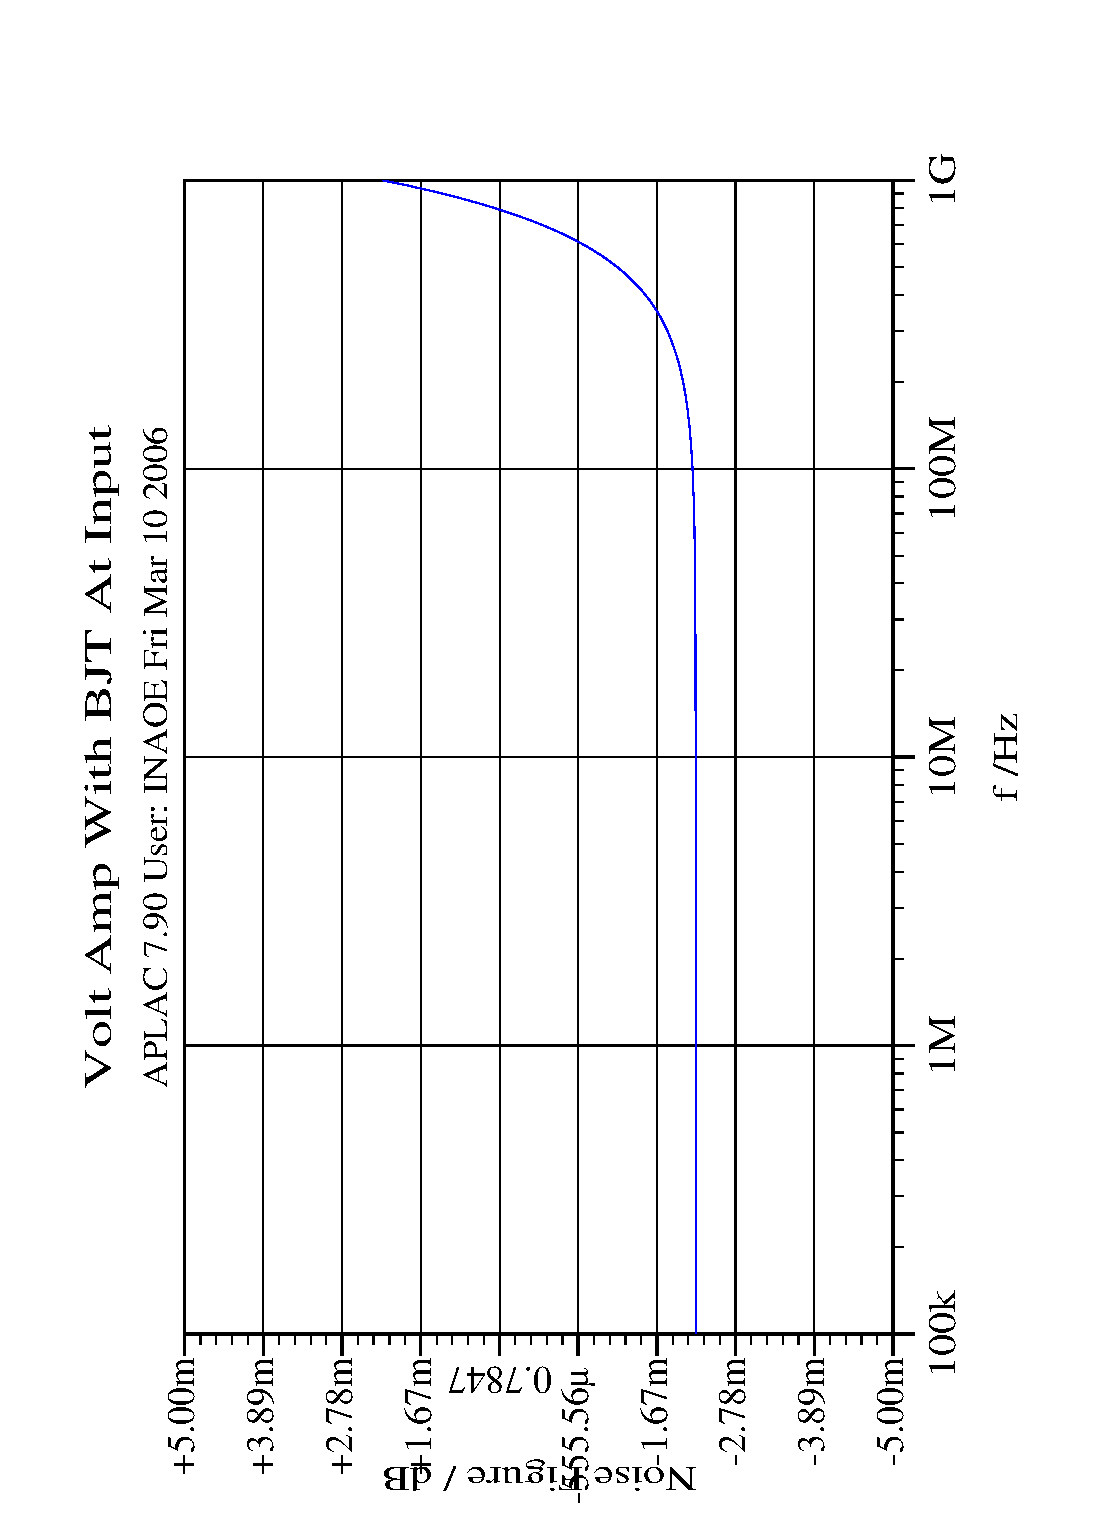
\includegraphics[scale=.3, angle=270]{figures/volt_amp_pi_1.eps}
	\caption{Frequency behaviour for voltage amplifier.}
	\label{figure10}
\end{figure}


\section{Conclusion}
This work has shown that is possible to perform the synthesis of nullor-based amplifiers by means of an automated tool. This tool rests on the foundations provided by the structure design methodology. A graphical interface makes possible to the designer perform the synthesis step-by-step through a wizard approach. Once the specification haven been given, the first synthesis equation are applied in order to calculate the feedback network value that fulfil the closed-loop gain while keeping the noise specs. The next step consists of the nullor synthesis, which is done by selecting an active device and a configuration. Herein the second synthesis formulae is applied to calculate the Ic-range that fulfils the permitted noise for the active part.

\section*{Acknowledgement}
Roberto Casta\~neda Sheissa is holder of a scholarship from CONACyT M\'exico under contract 118652/120341. This work has been supported by a CONACyT M\'exico research project under grant 42588-Y.


\bibliography{bib/midwest2006}
\end{document}


